\chapter{Bacteriologie: groei, fysiologie en genetica}\label{ch:b3:bacteriology}

Eén enkele cel van \emph{Escherichia coli} in warme bouillon deelt zich
elke twintig minuten. Ongehinderd zouden haar nakomelingen binnen twee
dagen zwaarder wegen dan de aarde; in werkelijkheid houden zij binnen
uren op, wanneer de suiker op is, en blijven zij wekenlang in een
toestand die de honger overleeft. Een verwante bacterie wordt, met een
wond en een paar uur, honderd miljoen cellen en koorts; honderd jaar
geleden doodde zij een derde van de patiënten die zij besmette, en
sinds 1941 heeft het gif van een schimmel ertegen meer levens gered dan
enig ander geneesmiddel --- terwijl de bacteriën in diezelfde tachtig
jaar wegen hebben gevonden om elk gemaakt \omterm{def:b3:bacteriology:antibiotics}{antibioticum} heen. Bacteriën
waren de organismen waarin voor het eerst werd aangetoond dat genen DNA
zijn, waarin de genregulatie voor het eerst werd begrepen, en waaraan
het gereedschap van \cref{ch:b3:genetic-engineering} is ontleend. Dit
hoofdstuk behandelt hen als organismen: hun omhulsel, de rekenkunde van
hun groei in een kolf en in een doorlopende kweek, de manier waarop een
populatie haar eigen dichtheid waarneemt, het verkeer van genen tussen
cellen, en de chemie en de evolutie van \omterm{def:b3:bacteriology:antibiotics}{antibiotica} en resistentie.

\section{De bacteriecel}

\begin{definition}[Het omhulsel]\label{def:b3:bacteriology:envelope}
\index{peptidoglycaan}\index{grampositief}\index{gramnegatief}\index{buitenmembraan}\index{lipopolysacharide}\index{endospore}
Op enkele na is elke bacterie omsloten door een wand van
\emph{peptidoglycaan}: ketens van afwisselend N-acetylglucosamine en
N-acetylmuraminezuur, door korte peptiden dwarsverbonden tot één
molecuul dat de cel omringt en de turgordruk van het cytoplasma ---
enkele atmosferen --- weerstaat. \emph{Grampositieve} bacteriën hebben
een dikke wand van \qtyrange{20}{80}{nm}, uit vele lagen, doorregen met
teichoïnezuren; \emph{gramnegatieve} bacteriën hebben een dunne wand
van één of twee lagen en daarbuiten een tweede lipidedubbellaag, het
\emph{buitenmembraan}, waarvan de buitenste laag uit
\emph{lipopolysacharide} bestaat (LPS, endotoxine --- het molecuul dat
het aangeboren afweersysteem van \cref{ch:b3:innate-immunity} herkent
en dat septische shock veroorzaakt), met daartussen een periplasma.
Porines in het buitenmembraan laten kleine moleculen door en houden
veel \omterm{def:b3:bacteriology:antibiotics}{antibiotica} buiten. Daarbuiten kunnen een polysacharidekapsel
tegen fagocyten liggen, zweepstaarten om te zwemmen
(\cref{ch:b3:cytoskeleton-motility}) en pili om te hechten en te
conjugeren. Binnenin is het chromosoom --- bij de meeste soorten één
cirkelvormig molecuul van \qtyrange{1}{10}{Mb} --- zonder membraan tot
een nucleoïde gevouwen, naast \omterm{def:b3:genetic-engineering:tools}{plasmiden}. Sommige geslachten
(\emph{Bacillus}, \emph{Clostridium}) kunnen een kopie van het
chromosoom in een dikke mantel sluiten als \emph{endospore},
uitgedroogd en stofwisselend inert, die koken, straling en eeuwen
droogte overleeft en ontkiemt zodra er weer voedingsstoffen zijn.
\end{definition}

\begin{method}[De gramkleuring]\label{met:b3:bacteriology:gram}
\index{gramkleuring}
De oudste toets in het bacteriologisch laboratorium (Gram, 1884)
bepaalt nog altijd de eerste keuze van \omterm{def:b3:bacteriology:antibiotics}{antibioticum}. (1) Strijk het
monster uit en fixeer het met warmte; (2) kleur met kristalviolet en
daarna met jodium, dat binnen de cellen een groot onoplosbaar complex
met de kleurstof vormt; (3) was met alcohol: het dikke \omterm{def:b3:bacteriology:envelope}{peptidoglycaan}
van \omterm{def:b3:bacteriology:envelope}{grampositieven}, door de alcohol uitgedroogd, houdt het complex
vast en de cellen blijven paars, terwijl de dunne wand van
\omterm{def:b3:bacteriology:envelope}{gramnegatieven} het eruit laat; (4) kleur na met safranine, dat de nu
kleurloze \omterm{def:b3:bacteriology:envelope}{gramnegatieven} roze maakt. Vorm en schikking --- kokken in
trossen (stafylokokken) of ketens (streptokokken), staafjes, spiralen
--- brengen de determinatie verder, en een paarse kok in trossen uit
een abces is een stafylokok nog voordat er een kweek is opgekomen.
\end{method}

\begin{omfigure}
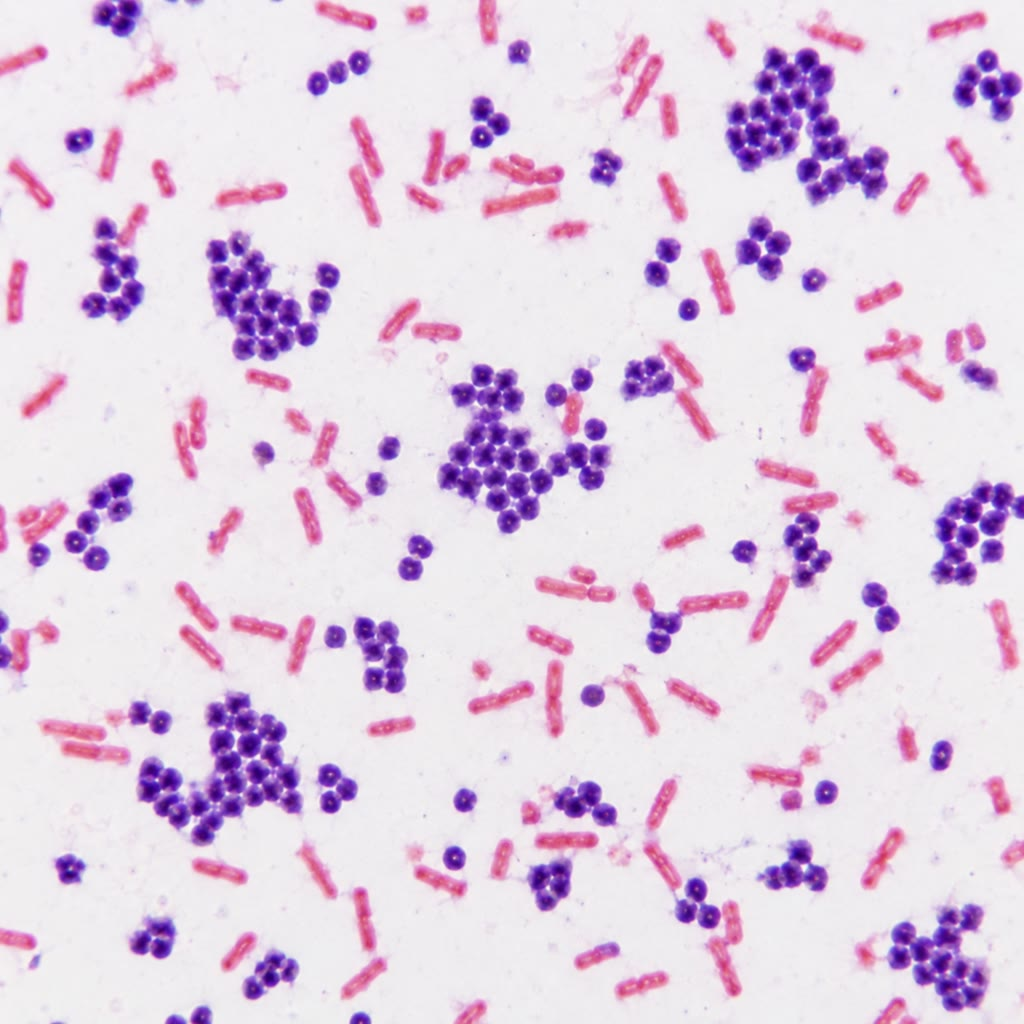
\includegraphics[width=0.36\linewidth]{images/book5/ai/b5-12-gram-stain.jpg}\hspace{0.04\linewidth}
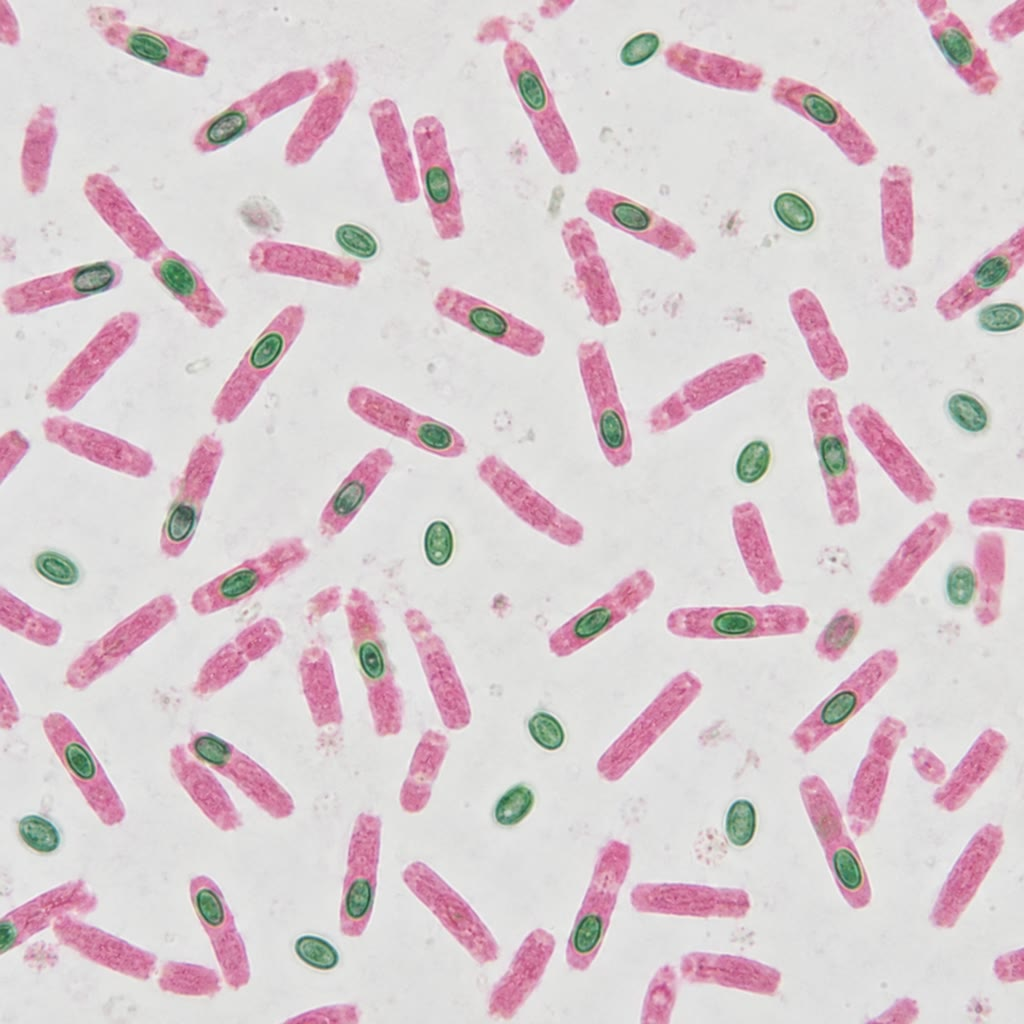
\includegraphics[width=0.36\linewidth]{images/book5/ai/b5-12-endospores.jpg}

{\small Links: een \omterm{met:b3:bacteriology:gram}{gramkleuring} --- paarse \omterm{def:b3:bacteriology:envelope}{grampositieve} kokken in
trossen, roze \omterm{def:b3:bacteriology:envelope}{gramnegatieve} staafjes. Rechts: cellen van
\emph{Bacillus} gekleurd voor \omterm{def:b3:bacteriology:envelope}{endosporen}, de heldergroene ovalen in
roze cellen en vrije sporen ernaast.}
\end{omfigure}

\begin{omfigure}
\begin{tikzpicture}[every node/.style={font=\scriptsize}, >=stealth]
  % Gram-positive
  \begin{scope}
    \fill[omDef!15] (0,0) rectangle (4.5,0.4); \draw[thick, omDef] (0,0) -- (4.5,0); \draw[thick, omDef] (0,0.4) -- (4.5,0.4);
    \fill[omProp!40] (0,0.5) rectangle (4.5,2.0); \foreach \y in {0.7,0.95,1.2,1.45,1.7} \draw[omProp!80!black, thin] (0,\y) -- (4.5,\y);
    \foreach \x in {0.6,1.6,2.6,3.6} \draw[omMeth!70!black, thick] (\x,0.5) -- (\x,2.3);
    \node[below] at (2.25,-0.1) {cytoplasmamembraan};
    \node[right, align=left] at (4.6,1.25) {dik peptidoglycaan\\(\qtyrange{20}{80}{nm})}; \node[right, omMeth!70!black] at (4.6,2.2) {teichoïnezuren};
    \node[above, font=\small\bfseries] at (2.25,2.5) {grampositief};
  \end{scope}
  % Gram-negative
  \begin{scope}[xshift=8.6cm]
    \fill[omDef!15] (0,0) rectangle (4.5,0.4); \draw[thick, omDef] (0,0) -- (4.5,0); \draw[thick, omDef] (0,0.4) -- (4.5,0.4);
    \fill[omProp!40] (0,0.75) rectangle (4.5,1.05); \draw[omProp!80!black, thin] (0,0.9) -- (4.5,0.9);
    \fill[omDef!15] (0,1.5) rectangle (4.5,1.9); \draw[thick, omDef] (0,1.5) -- (4.5,1.5); \draw[thick, omDef] (0,1.9) -- (4.5,1.9);
    \foreach \x in {0.4,0.9,1.4,1.9,2.4,2.9,3.4,3.9} \draw[omThm, thick] (\x,1.9) -- (\x,2.35);
    \draw[thick, fill=white] (2.0,1.45) rectangle (2.5,1.95); \node[below, font=\tiny] at (2.25,1.45) {porine};
    \node[below] at (2.25,-0.1) {cytoplasmamembraan};
    \node[right] at (4.6,0.9) {dun peptidoglycaan}; \node[right] at (4.6,1.7) {buitenmembraan}; \node[right, omThm] at (4.6,2.25) {LPS (endotoxine)};
    \node[right, font=\tiny] at (4.6,1.27) {periplasma};
    \node[above, font=\small\bfseries] at (2.25,2.5) {gramnegatief};
  \end{scope}
\end{tikzpicture}

{\small De twee omhulsels. \omterm{def:b3:bacteriology:envelope}{Grampositieven} wikkelen het membraan in vele
lagen \omterm{def:b3:bacteriology:envelope}{peptidoglycaan}; \omterm{def:b3:bacteriology:envelope}{gramnegatieven} hebben een dunne laag en een
\omterm{def:b3:bacteriology:envelope}{buitenmembraan} van \omterm{def:b3:bacteriology:envelope}{lipopolysacharide}, doorboord door porines, dat veel
\omterm{def:b3:bacteriology:antibiotics}{antibiotica} buiten houdt en het endotoxine levert dat septische shock
veroorzaakt.}
\end{omfigure}

\section{Groei}

\begin{theorem}[Exponentiële groei, de wet van Monod en de chemostaat]\label{thm:b3:bacteriology:monod}
\index{exponentiële groei!bacteriën}\index{vergelijking van Monod}\index{chemostaat}\index{verdunningssnelheid}
Een populatie van $N$ cellen die zich met generatietijd $T$ deelt
groeit als $N(t) = N_{0}\,2^{t/T} = N_{0}e^{\mu t}$ met specifieke groeisnelheid $\mu =
\ln 2/T$. De snelheid hangt van de beperkende voedingsstof $S$ af
volgens de \emph{wet van Monod}
\[
\mu(S) = \mu_{\max}\,\frac{S}{K_{S} + S},
\]
die bij $\mu_{\max}$ verzadigt en half maximaal is bij $S = K_{S}$. In
een \emph{chemostaat} --- een vat van volume $V$ waarin vers medium met
een voedingsstofconcentratie $S_{0}$ met snelheid $F$ instroomt en
waaruit kweek met dezelfde snelheid vertrekt, met \omterm{thm:b3:bacteriology:monod}{verdunningssnelheid}
$D = F/V$ --- geldt in evenwicht
\[
\mu(S^{*}) = D,\qquad S^{*} = \frac{K_{S}D}{\mu_{\max} - D},\qquad
X^{*} = Y\,(S_{0} - S^{*}),
\]
waarin $X$ de celdichtheid is en $Y$ de opbrengst (cellen gemaakt per
eenheid voedingsstof). De onderzoeker stelt de groeisnelheid in door
aan een pomp te draaien; de kweek antwoordt door de voedingsstof aan te
passen die zij achterlaat. Overschrijdt $D$ de waarde $\mu(S_{0})$, dan
kunnen de cellen het niet bijhouden en worden zij uitgespoeld.
\end{theorem}
\begin{proof}
Cellen: $\mathrm{d}X/\mathrm{d}t = \mu(S)X - DX$, groei min uitstroom;
in evenwicht met $X^{*} > 0$ geldt $\mu(S^{*}) = D$, en de wet van
Monod omkeren geeft $S^{*}$. Voedingsstof:
$\mathrm{d}S/\mathrm{d}t = D(S_{0} -
S) - \mu(S)X/Y$, instroom min uitstroom min verbruik; in evenwicht, met
$\mu = D$, geldt $D(S_{0} - S^{*}) = DX^{*}/Y$, waaruit $X^{*}$ volgt.
De evenwichtstoestand bestaat alleen als $S^{*} < S_{0}$, dat wil
zeggen $D <
\mu(S_{0})$; daarboven is de enige evenwichtstoestand $X = 0$,
uitspoeling. Stabiliteit: stijgt $X$ boven $X^{*}$, dan verbruikt zij
meer, zakt $S$ onder $S^{*}$, zakt $\mu$ onder $D$ en neemt $X$ af ---
een negatieve terugkoppeling via de voedingsstof.
\end{proof}

\begin{example}[Een kweek in getallen]\label{ex:b3:bacteriology:numbers}
\emph{E.~coli} in rijk medium bij \qty{37}{\celsius}: $T = \qty{20}{min}$,
$\mu = \qty{2.1}{h^{-1}}$. Vanuit één cel na twaalf uur $2^{36}$ ---
$7\times 10^{10}$ cellen, ongeveer \qty{70}{mg}, en daar houdt een kolf
van \qty{100}{mL} op bij gebrek aan zuurstof en suiker; ``de massa van
de aarde in twee dagen'' is $2^{144}\approx 10^{43}$ cellen, en de
rekensom laat alleen zien dat exponentiële groei nooit voortduurt. In
een chemostaat op glucose met $\mu_{\max} = \qty{1.0}{h^{-1}}$, $K_{S} =
\qty{0.01}{g/L}$, $S_{0} = \qty{1}{g/L}$ en $Y = \qty{0.5}{g}$ cellen
per gram glucose laat een \omterm{thm:b3:bacteriology:monod}{verdunningssnelheid} van \qty{0.5}{h^{-1}}
$S^{*}
= 0.01\times 0.5/0.5 = \qty{0.01}{g/L}$ glucose over en houdt zij $X^{*} =
\qty{0.495}{g/L}$ cellen vast, die zich onbeperkt elke \qty{83}{min}
delen. Met de chemostaat wordt de fysiologie bij een
vaste groeisnelheid bestudeerd, en worden duizenden generaties evolutie
in een fles doorlopen.
\end{example}

\begin{omfigure}
\begin{tikzpicture}
\begin{axis}[
  width=6.6cm, height=5.4cm,
  axis x line=bottom, axis y line=left,
  xmin=0, xmax=14, ymin=1e6, ymax=1e10, ymode=log,
  xlabel={uren}, ylabel={cellen per mL},
  xlabel style={font=\small, at={(axis description cs:0.5,-0.12)}, anchor=north}, ylabel style={font=\small},
  tick label style={font=\scriptsize}, xtick={0,4,8,12},
  clip=false,
]
\addplot[very thick, omDef, domain=0:1.5, samples=2] {1e6};
\addplot[very thick, omDef, domain=1.5:7.5, samples=40] {1e6*2^((x-1.5)/0.5)};
\addplot[very thick, omDef, domain=7.5:12, samples=2] {4.1e9};
\addplot[very thick, omDef, domain=12:14, samples=10] {4.1e9*exp(-0.15*(x-12))};
\node[font=\scriptsize, anchor=south] at (axis cs:0.8,1.2e6) {vertraging};
\node[font=\scriptsize, anchor=west] at (axis cs:2.5,3e8) {exponentieel: $T = \qty{30}{min}$};
\node[font=\scriptsize, anchor=north] at (axis cs:10,3.5e9) {stationair};
\node[font=\scriptsize, anchor=north] at (axis cs:12.8,2.2e9) {sterfte};
\end{axis}
\begin{axis}[
  at={(7.8cm,0)}, anchor=south west,
  width=6.6cm, height=5.4cm,
  axis x line=bottom, axis y line=left,
  xmin=0, xmax=0.1, ymin=0, ymax=1.1,
  xlabel={glucose $S$ (g/L)}, ylabel={$\mu$ (h$^{-1}$)},
  xlabel style={font=\small, at={(axis description cs:0.5,-0.12)}, anchor=north}, ylabel style={font=\small},
  tick label style={font=\scriptsize}, xtick={0,0.01,0.05,0.1}, xticklabels={0,$K_S$,0.05,0.1}, ytick={0,0.5,1},
  clip=false,
]
\addplot[very thick, omThm, domain=0:0.1, samples=60] {x/(0.01+x)};
\addplot[dashed, gray, domain=0:0.1, samples=2] {1};
\addplot[dashed, gray] coordinates {(0.01,0) (0.01,0.5)}; \addplot[dashed, gray] coordinates {(0,0.5) (0.01,0.5)};
\node[font=\scriptsize, omThm, anchor=north west] at (axis cs:0.045,0.6) {Monod: $\mu = \mu_{\max}S/(K_{S}+S)$};
\node[font=\scriptsize, gray, anchor=south east] at (axis cs:0.1,1.01) {$\mu_{\max}$};
\end{axis}
\end{tikzpicture}

{\small Links: een kweek in een kolf --- een vertraging terwijl de
enzymen worden aangezet, exponentiële groei, een \omterm{def:b3:bacteriology:phases}{stationaire fase}
wanneer de voedingsstof op is, en trage sterfte. Rechts: de wet van
Monod, de groeisnelheid tegen de beperkende voedingsstof, met $K_{S}$
de concentratie voor half maximale groei.}
\end{omfigure}

\begin{definition}[Fasen en toestanden]\label{def:b3:bacteriology:phases}
\index{vertragingsfase}\index{stationaire fase}\index{sporulatie}\index{sigmafactor}
In een verse kolf (een \emph{kweek in een gesloten vat}) pauzeren de
cellen eerst --- de \emph{vertragingsfase}, terwijl zij de enzymen
aanzetten die het nieuwe medium vraagt --- groeien zij daarna
exponentieel, en houden zij op zodra een voedingsstof op is of een
afvalstof zich ophoopt: de \emph{stationaire fase}, waarin de cellen
krimpen, hun omhulsel verdikken, hun nucleoïde om beschermende eiwitten
samenpakken, via de alternatieve sigmafactor RpoS hun stressgenen
aanzetten, en maanden kunnen overleven; daarna volgt een sterftefase
waarin de meeste cellen uiteenvallen en enkele op de resten
verderleven. Sommige soorten beantwoorden de honger met een
ontwikkelingsprogramma: \emph{Bacillus subtilis} deelt zich asymmetrisch
en de grotere cel verzwelgt de kleinere en bouwt de spore eromheen, een
reeks van acht uur die wordt bestuurd door een cascade van
\emph{sigmafactoren} --- de subeenheden die het RNA-polymerase naar één
stel promotoren sturen --- afwisselend in de twee compartimenten, het
eerste bacteriële voorbeeld van differentiatie en van signalering van
cel tot cel door een wand heen.
\end{definition}

\section{Elkaar waarnemen}

\begin{definition}[Quorumdetectie]\label{def:b3:bacteriology:quorum}
\index{quorumdetectie}\index{auto-inductor}\index{tweecomponentensysteem}
Bacteriën nemen hun eigen dichtheid waar met \emph{quorumdetectie}:
elke cel scheidt met een constante snelheid een klein signaalmolecuul
af, een \emph{auto-inductor} --- geacyleerde homoserinelactonen bij
\omterm{def:b3:bacteriology:envelope}{gramnegatieven}, korte peptiden bij \omterm{def:b3:bacteriology:envelope}{grampositieven} ---; de concentratie
in het medium stijgt met het aantal cellen, en zodra zij een drempel
overschrijdt bindt zij een receptor die een stel genen aanzet, waaronder
het synthase van de auto-inductor zelf (vandaar de naam). De genen die
zo worden bestuurd zijn die welke alleen in gezelschap lonen: licht bij
\emph{Vibrio fischeri}, virulentiefactoren bij \emph{Staphylococcus
aureus} en \emph{Pseudomonas aeruginosa}, de matrix van een biofilm, de
bekwaamheid om DNA op te nemen, en het doden van buren. Het meeste
waarnemen bij bacteriën verloopt via \emph{tweecomponentensystemen}:
een histidinekinase in het membraan dat een prikkel bemerkt en een
responsregulator in het cytoplasma fosforyleert, die DNA bindt --- een
cel heeft er tientallen, voor fosfaat, osmolariteit, zuurstof en de
auto-inductoren van andere soorten.
\end{definition}

\begin{proof}[Bewijsmateriaal]
Nealson, Platt en Hastings (1970) kweekten de lichtgevende
zeebacterie \emph{Vibrio fischeri} uit een verdund entsel en vonden dat
de cellen geen licht maakten tot zij een dichtheid van zo'n $10^{7}$
per milliliter bereikten, waarna zij allemaal tegelijk oplichtten;
medium waarin een dichte kweek was gegroeid, gesteriliseerd en aan een
verdunde kweek toegevoegd, zette het licht meteen aan. De cellen telden
een afgescheiden stof, niet de tijd of de voeding. De stof werd
geïdentificeerd als een acylhomoserinelacton (Eberhard, 1981), en de
genen --- \emph{luxI} voor het synthase, \emph{luxR} voor de receptor,
en het luciferase-operon dat zij besturen --- werden in \emph{E.~coli}
gekloneerd, dat toen bij dichtheid oplichtte. In de inktvis die de
bacterie bij $10^{10}$ per milliliter huisvest schijnt het lichtorgaan;
in zee, waar de bacteriën verdund zijn, zijn zij donker en besparen zij
de kosten.
\end{proof}

\begin{proposition}[Een dichtheidsdrempel]\label{prop:b3:bacteriology:threshold}
\index{quorumdetectie!drempel}
Laat elk van $N$ cellen in een volume $V$ \omterm{def:b3:bacteriology:quorum}{auto-inductor} afscheiden met
snelheid $p$ moleculen per seconde, en laat het molecuul met
eerste-ordesnelheid $k$ verloren gaan (afgebroken of verdund). De
concentratie nadert $A^{*} = pN/(kV)$, evenredig met de celdichtheid
$N/V$, met tijdconstante $1/k$; de receptor gaat aan wanneer $A^{*}$
zijn drempel $A_{\text{thr}}$ bereikt, dat wil zeggen bij de dichtheid
\[
\left(\frac{N}{V}\right)_{\text{thr}} = \frac{k\,A_{\text{thr}}}{p}.
\]
In een afgesloten ruimte --- het lichtorgaan van een inktvis, een
abces, het slijm van een long --- is $k$ klein omdat het signaal niet
wordt afgevoerd, zodat de drempeldichtheid door minder cellen wordt
gehaald; in open water wordt zij nooit gehaald. De cel meet dus niet
haar aantal maar haar aantal per eenheid van het volume dat zij deelt,
en dat is wat telt voor elke gezamenlijke daad; de positieve
terugkoppeling van de \omterm{def:b3:bacteriology:quorum}{auto-inductor} op zijn eigen synthase maakt de
schakeling scherp: zodra enkele cellen de drempel overschrijden, duwt
hun extra uitstoot de rest eroverheen.
\end{proposition}
\begin{proof}
$\mathrm{d}A/\mathrm{d}t = pN/V - kA$ heeft de evenwichtstoestand
$A^{*} =
pN/(kV)$ en nadert die als $e^{-kt}$. Stelt men $A^{*} = A_{\text{thr}}$
en lost men naar $N/V$ op, dan volgt de drempeldichtheid.
\end{proof}

\begin{omfigure}
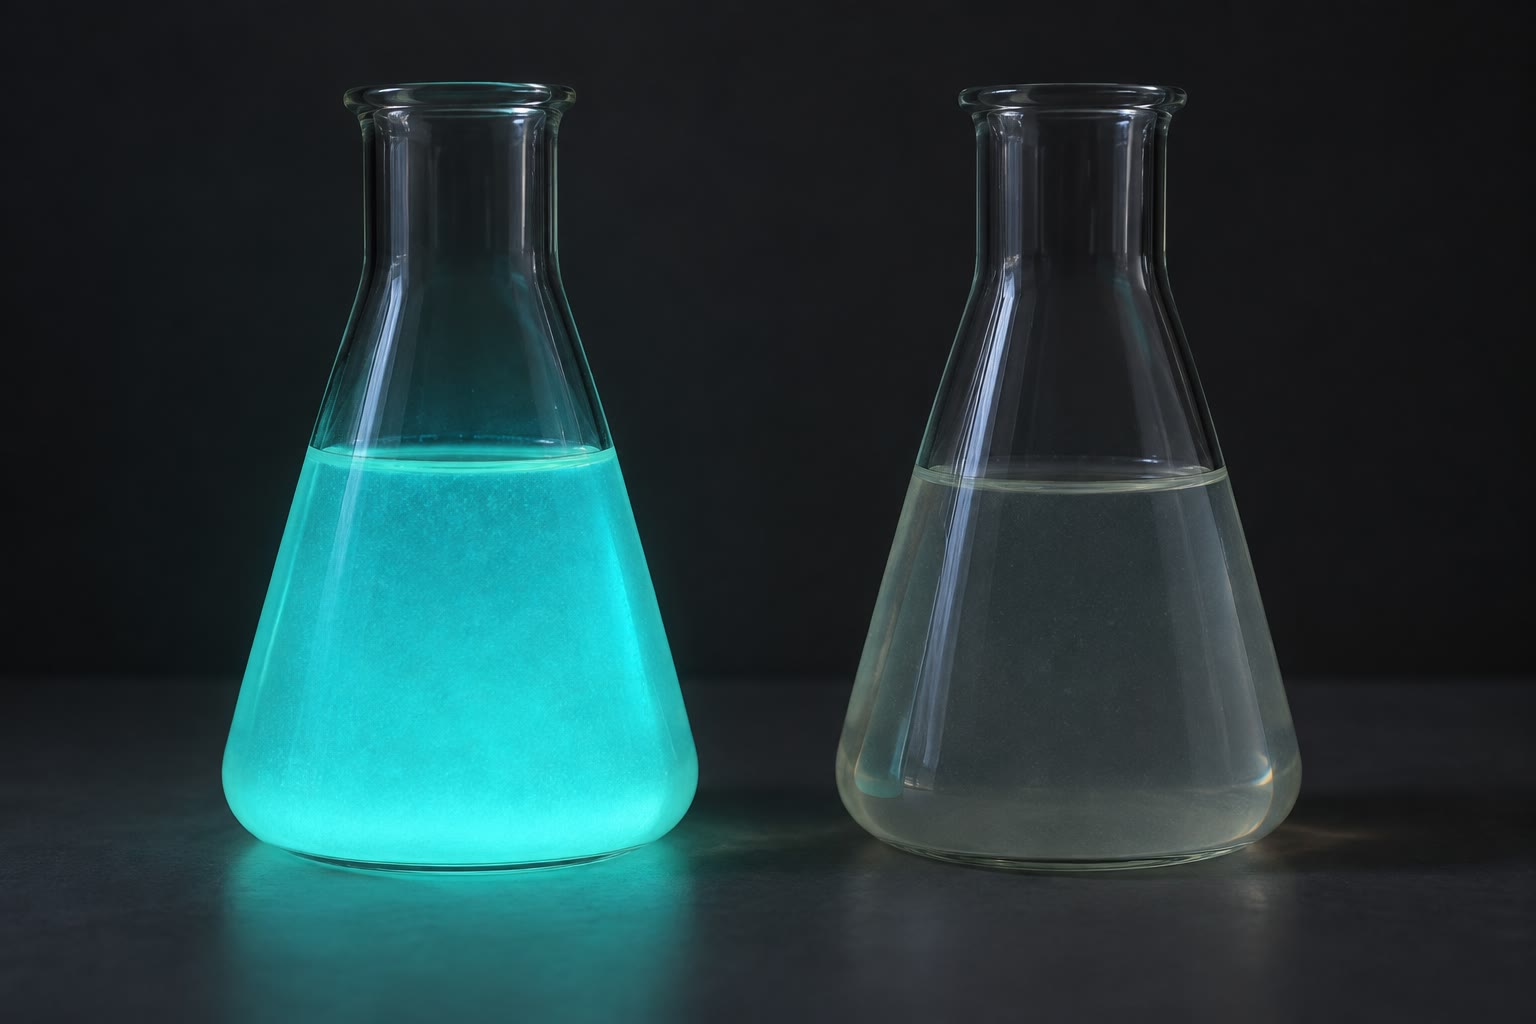
\includegraphics[width=0.46\linewidth]{images/book5/ai/b5-12-quorum-glow.jpg}\hspace{0.04\linewidth}
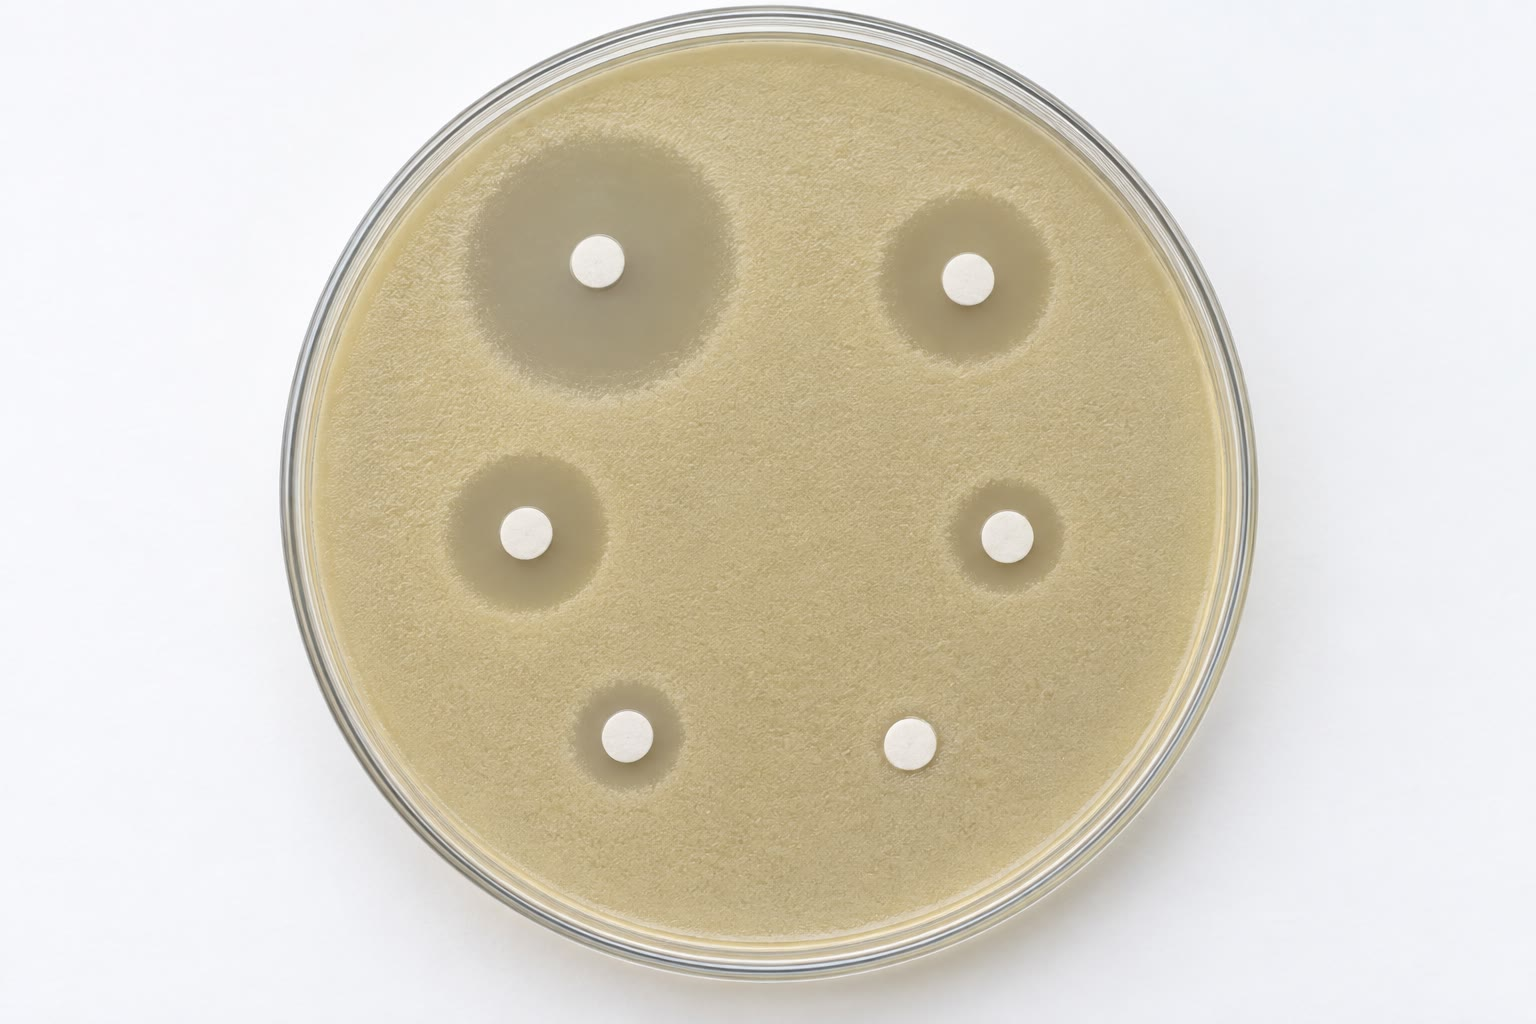
\includegraphics[width=0.46\linewidth]{images/book5/ai/b5-12-antibiotic-disks.jpg}

{\small Links: een dichte kweek van \emph{Vibrio fischeri} die
oplicht, naast een verdunde die donker is --- dezelfde cellen, boven en
onder hun quorum. Rechts: een schijfjestest; de diameter van elke
heldere zone meet de gevoeligheid van de bacterie voor het \omterm{def:b3:bacteriology:antibiotics}{antibioticum}
op dat schijfje, en het schijfje zonder zone wijst op resistentie.}
\end{omfigure}

\section{Het verkeer van genen}

\begin{definition}[Horizontale genoverdracht]\label{def:b3:bacteriology:hgt}
\index{transformatie}\index{transductie}\index{conjugatie}\index{plasmide!resistentie}\index{mobiel genetisch element}\index{pangenoom}
Bacteriën planten zich klonaal voort maar wisselen genen uit langs drie
wegen. De \emph{transformatie}: de opname van naakt DNA uit de omgeving
door een bekwame cel --- de weg waarlangs de pneumokokken van Griffith
hun kapsel kregen en waarlangs Avery aantoonde dat het transformerende
beginsel DNA was (1944). De \emph{transductie}: een faag die een stuk
gastheer-DNA inpakt en in de volgende gastheer spuit
(\cref{ch:b3:virology}). De \emph{conjugatie}: de overdracht van een
\omterm{def:b3:genetic-engineering:tools}{plasmide} door een pilus en een paringsbrug van een donor die het draagt
naar een ontvanger, aangetoond door Lederberg en Tatum (1946) met
auxotrofe stammen van \emph{E.~coli} die alleen prototrofe
recombinanten opleverden wanneer zij werden gemengd. Conjugatieve
\omterm{def:b3:genetic-engineering:tools}{plasmiden} dragen hun eigen overdrachtsgenen; veel dragen ook
resistentiegenen, vaak samengebracht in \emph{integronen} en geflankeerd
door transposons, zodat één paring resistentie tegen vijf \omterm{def:b3:bacteriology:antibiotics}{antibiotica}
tegelijk kan overdragen, over de soortgrens heen. Het gevolg is dat een
bacteriesoort een kerngenoom heeft dat alle stammen delen en een
aanvullend genoom dat verschilt --- een \emph{pangenoom}: twee stammen
van \emph{E.~coli} kunnen in een vijfde van hun genen verschillen, en
ziekteverwekkende stammen verschillen van onschuldige vooral door
verworven eilanden met virulentiegenen. De genen van het
mutatiehoofdstuk uit het boek van jaar~2 ontstaan door mutatie; de
genen van dit hoofdstuk arriveren meestal.
\end{definition}

\begin{omfigure}
\begin{tikzpicture}[every node/.style={font=\scriptsize}, >=stealth]
  % transformation
  \begin{scope}
    \draw[thick, fill=omDef!15] (0,0) ellipse (1.0 and 0.55);
    \draw[omThm, very thick] (-1.9,0.6) .. controls (-1.5,0.8) .. (-1.2,0.5); \draw[->, omThm, thick] (-1.2,0.5) -- (-0.7,0.25);
    \node[below, align=center] at (0,-0.7) {transformatie:\\naakt DNA opgenomen\\door een bekwame cel};
  \end{scope}
  % transduction
  \begin{scope}[xshift=4.6cm]
    \draw[thick, fill=omDef!15] (0,0) ellipse (1.0 and 0.55);
    \draw[thick, fill=omProp!40] (-1.3,1.0) -- (-1.0,1.3) -- (-0.7,1.0) -- (-1.0,0.7) -- cycle; \draw[thick] (-1.0,0.7) -- (-0.9,0.35);
    \draw[omThm, very thick] (-1.1,1.15) -- (-0.9,0.85);
    \node[below, align=center] at (0,-0.7) {transductie:\\een faag draagt een stuk DNA\\van zijn vorige gastheer};
  \end{scope}
  % conjugation
  \begin{scope}[xshift=9.6cm]
    \draw[thick, fill=omDef!15] (-1.3,0) ellipse (0.9 and 0.5); \draw[thick, fill=omDef!15] (1.3,0) ellipse (0.9 and 0.5);
    \draw[very thick, omMeth!70!black] (-0.4,0) -- (0.4,0);
    \draw[omThm, very thick] (-1.5,0) circle (0.25); \draw[->, omThm, thick] (-1.25,0) -- (1.0,0);
    \node[below, align=center] at (0,-0.7) {conjugatie:\\een plasmide steekt\\een paringsbrug over};
  \end{scope}
\end{tikzpicture}

{\small De drie wegen van horizontale overdracht. Genen voor
resistentie, virulentie en stofwisseling verhuizen tussen cellen --- en
tussen soorten --- sneller dan de mutatie ze zou kunnen maken.}
\end{omfigure}

\begin{proof}[Bewijsmateriaal]
Robert Koch (1876--1884) stelde vast dat een bepaalde bacterie een
bepaalde ziekte veroorzaakt: hij isoleerde \emph{Bacillus anthracis}
uit zieke dieren, kweekte haar zuiver op een vaste bodem (de agarplaat
en de enkele kolonie zijn uitvindingen van zijn laboratorium), toonde
aan dat de kweek miltvuur in gezonde dieren opwekte en er weer uit te
isoleren viel --- de postulaten die een ziekteverwekker nog altijd
bepalen --- en ging daarna door met de tuberkelbacil en de
choleravibrio. Alexander Fleming (1928) merkte op dat een schimmel die
een plaat met stafylokokken had verontreinigd een heldere zone om zich
heen had gemaakt; de stof, penicilline, werd gezuiverd en Florey en
Chain (1940--1941) toonden aan dat zij infecties genas, en binnen een
decennium waren resistente stafylokokken met een enzym dat penicilline
vernietigt gewoon in ziekenhuizen --- een waarschuwing die Fleming zelf
in zijn Nobellezing gaf.
\end{proof}

\begin{omfigure}
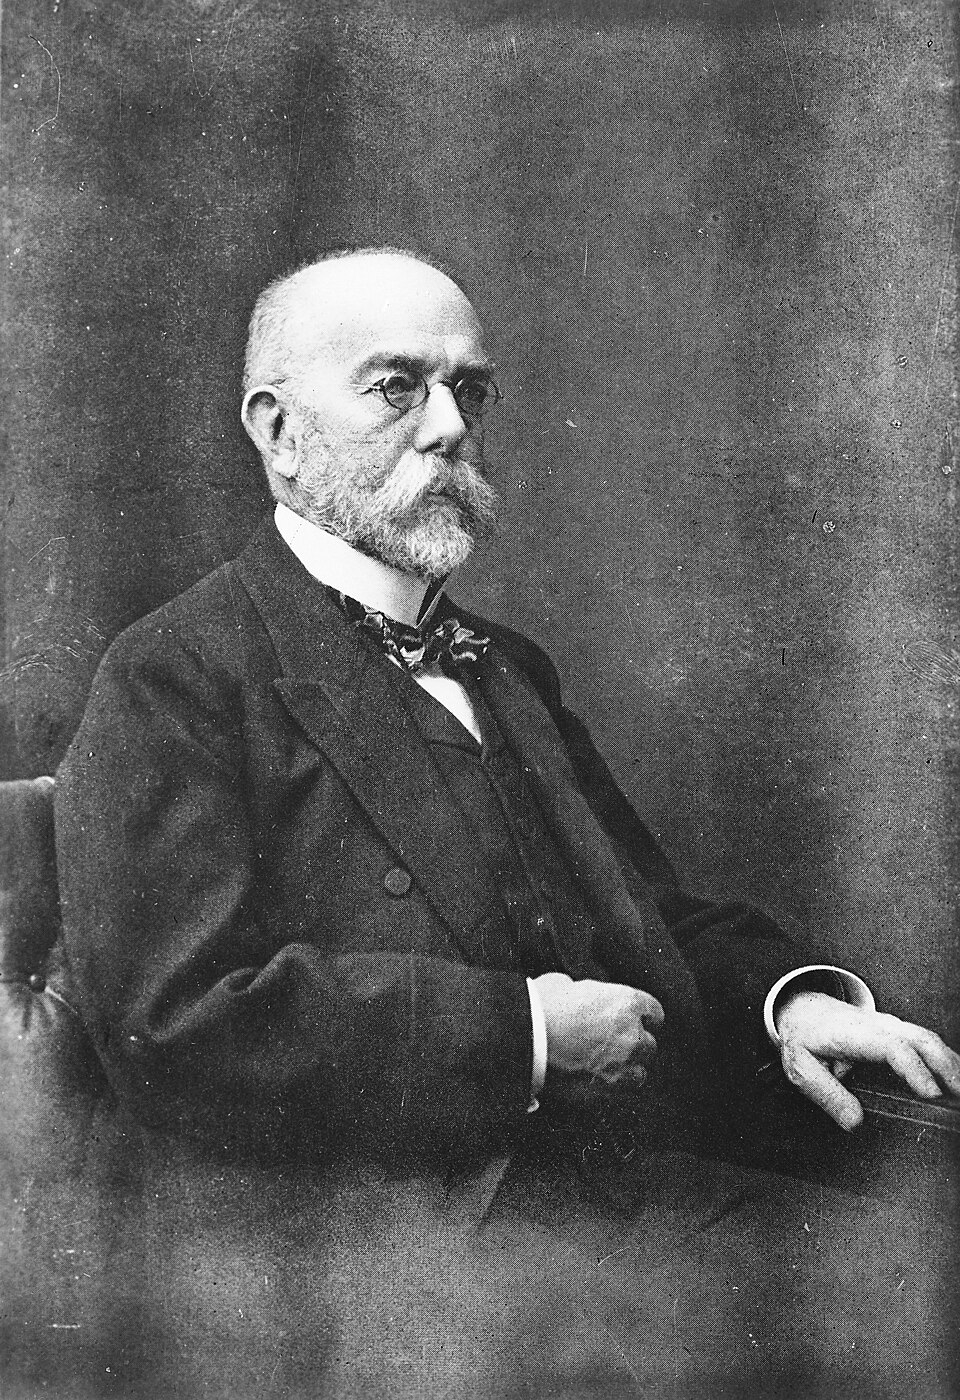
\includegraphics[width=0.30\linewidth]{images/book5/koch.jpg}\hspace{0.04\linewidth}
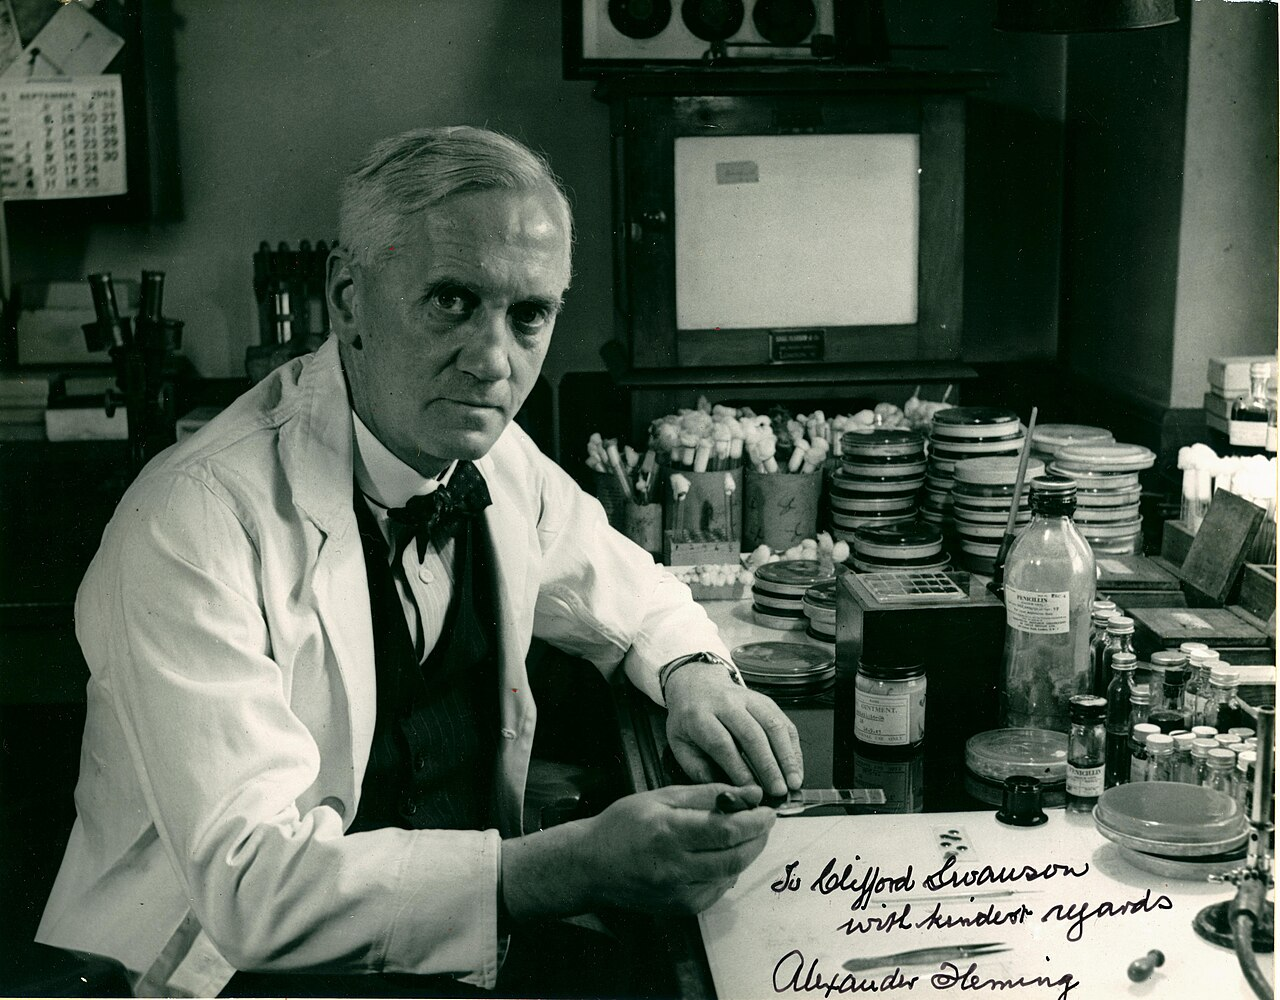
\includegraphics[width=0.56\linewidth]{images/book5/fleming.jpg}

{\small Robert Koch, die bewees dat bepaalde bacteriën bepaalde ziekten
veroorzaken en de methoden bedacht om ze te kweken (Wellcome
Collection, CC~BY~4.0). Rechts: Alexander Fleming in zijn laboratorium
met platen van de schimmel waarvan het product penicilline werd (archief
van de Amerikaanse marine, publiek domein).}
\end{omfigure}

\section{Antibiotica en resistentie}

\begin{definition}[Antibiotica]\label{def:b3:bacteriology:antibiotics}
\index{antibioticum}\index{bètalactam}\index{selectieve toxiciteit}\index{minimaal remmende concentratie}
Een \emph{antibioticum} is een molecuul dat bacteriën doodt of hun
groei stopt bij concentraties die voor de gastheer onschadelijk zijn,
door in te grijpen op een doelwit dat de gastheer niet heeft of in een
andere vorm heeft --- de \emph{selectieve toxiciteit}. De doelwitten
zijn weinig talrijk. De celwand: de \emph{$\beta$-lactams}
(penicillines, cefalosporines, carbapenems) bootsen het eindstandige
D-Ala-D-Ala van het peptide van het \omterm{def:b3:bacteriology:envelope}{peptidoglycaan} na en acyleren de
enzymen die het dwarsverbinden, zodat de groeiende wand zwak is en de
cel onder haar eigen turgor barst; vancomycine bindt het D-Ala-D-Ala
zelf. Het ribosoom, waarvan de bacteriële vorm van de eukaryote
verschilt: de aminoglycosiden (de kleine subeenheid, wat verkeerd lezen
veroorzaakt), de tetracyclines (die de intrede van tRNA blokkeren), de
macroliden en chlooramfenicol (de uitgangstunnel en het
peptidyltransferase van de grote subeenheid). Het DNA-gyrase en
topo-isomerase~IV: de chinolonen. Het RNA-polymerase: rifampicine. De
foliumzuursynthese, die dieren niet doen: de sulfonamiden en
trimethoprim. Het membraan: de polymyxines, een laatste redmiddel. De
\emph{minimaal remmende concentratie} (MRC) is de laagste concentratie
van een middel die zichtbare groei van een stam verhindert; een stam
heet resistent wanneer haar MRC hoger ligt dan de concentratie die het
middel in de patiënt haalt.
\end{definition}

\begin{method}[Gevoeligheid meten]\label{met:b3:bacteriology:mic}
\index{schijfjesdiffusie}\index{bouillonverdunning}
Twee toetsen. De \emph{\omterm{met:b3:bacteriology:mic}{bouillonverdunning}}: ent een vast aantal cellen
(ongeveer $5\times 10^{5}$ per milliliter) in een rij buisjes of putjes
met het \omterm{def:b3:bacteriology:antibiotics}{antibioticum} in stappen van twee, laat een nacht groeien, en
lees het eerste heldere putje af: die concentratie is de MRC. De
\emph{schijfjesdiffusie}: strijk de stam op een agarplaat uit, leg er
papieren schijfjes met bekende hoeveelheden van verscheidene
\omterm{def:b3:bacteriology:antibiotics}{antibiotica} op, en laat groeien; het middel diffundeert naar buiten, de
concentratie daalt met de afstand, en de groei wordt geremd tot de
straal waar de concentratie de MRC is, zodat de diameter van de
heldere zone --- afgelezen tegen geijkte tabellen --- op één plaat de
gevoeligheid voor elk schijfje geeft. Beide toetsen kosten een dag; het
genoom sequencen op bekende resistentiegenen en mutaties kost dezelfde
dag en begint ze te vervangen.
\end{method}

\begin{definition}[Resistentie]\label{def:b3:bacteriology:resistance}
\index{antibioticaresistentie}\index{bètalactamase}\index{effluxpomp}\index{MRSA}
Een bacterie weerstaat een \omterm{def:b3:bacteriology:antibiotics}{antibioticum} op een van vijf manieren. Zij
vernietigt het middel: de \emph{$\beta$-lactamasen} hydrolyseren de
$\beta$-lactamring, en de varianten met verbreed spectrum en de
carbapenemasen vernietigen nu ook de nieuwste. Zij verandert het
doelwit: een mutatie in het ribosomale eiwit of het gyrase dat het
middel bindt, of, bij MRSA (methicillineresistente
\emph{Staphylococcus aureus}), een verworven gen voor een
dwarsverbindend enzym dat de $\beta$-lactams niet binden; de
resistentie tegen vancomycine vervangt het eindstandige D-Ala door
D-lactaat, dat het middel niet herkent. Zij pompt het middel naar
buiten met \emph{effluxpompen}, vaak met een brede specificiteit. Zij
verhindert dat het middel binnenkomt, door een porine te verliezen. Of
zij omzeilt de geblokkeerde stap met een ander enzym.
Doelwitmutaties ontstaan bij toeval in de patiënt met snelheden van
$10^{-8}$ tot $10^{-6}$ per deling en worden tijdens de behandeling
geselecteerd; de enzymen en de pompen worden meestal op \omterm{def:b3:genetic-engineering:tools}{plasmiden}
verworven uit het enorme reservoir van bodem- en darmbacteriën, waarin
zij in de loop van tijdperken zijn ontstaan tegen de \omterm{def:b3:bacteriology:antibiotics}{antibiotica} die
schimmels en andere bacteriën maken. Persisters --- sluimerende cellen
die een middel overleven zonder genetisch resistent te zijn ---
verklaren de terugval na een behandeling die had moeten werken.
\end{definition}

\begin{proposition}[Waarom resistentie onvermijdelijk is en de combinatie het antwoord]\label{prop:b3:bacteriology:selection}
\index{resistentie!selectie}\index{combinatietherapie!antibiotica}
Een infectie van $10^{9}$ cellen die wordt behandeld met een middel
waartegen resistentiemutaties met $10^{-8}$ per deling ontstaan bevat
al ongeveer tien resistente cellen; het middel doodt de rest en die
tien nemen het over --- precies de rekenkunde van
\cref{ch:b3:cancer-biology}, omdat een bacteriepopulatie en een \omterm{def:b3:cancer-biology:hallmarks}{tumor}
beide evoluerende klonen onder selectie zijn. Twee middelen met
onafhankelijke doelwitten staan tegenover een dubbel resistente cel bij
$10^{-16}$ per deling, en die bevat een miljard cellen niet. Daarom
wordt de tuberculose, waarvan de haarden $10^{8}$--$10^{9}$ bacillen
bevatten, sinds de jaren vijftig met drie of vier middelen tegelijk
behandeld, en daarom bracht behandeling met één middel binnen maanden
resistentie voort; en daarom selecteert elk gebruik van een
\omterm{def:b3:bacteriology:antibiotics}{antibioticum}, bij een patiënt of in een mestbedrijf, ergens
resistentie, en is het tempo van nieuwe \omterm{def:b3:bacteriology:antibiotics}{antibiotica} --- sinds de jaren
zestig geen enkele nieuwe klasse tegen \omterm{def:b3:bacteriology:envelope}{gramnegatieven} --- de maat
waartegen de verliezen worden geteld. De remedies zijn die van elke
evolutionaire wedstrijd: gebruik minder, combineer, maak de kuur af
zodat deels resistente cellen niet overleven om zich voort te planten,
en zoek nieuwe doelwitten.
\end{proposition}

\begin{example}[Het venster van de mutantselectie]\label{ex:b3:bacteriology:window}
Een stam heeft een MRC van \qty{1}{mg/L}; haar resistente mutanten van
de eerste stap, die in één op $10^{7}$ aanwezig zijn, hebben een MRC van
\qty{8}{mg/L}. Een dosis die het middel op \qty{4}{mg/L} houdt doodt het
wildtype en laat de mutanten zonder concurrentie groeien: het
concentratiegebied tussen de MRC van het wildtype en die van de
mutanten is het \emph{venster van de mutantselectie}, en een
behandeling die daarin blijft kweekt resistentie. Een dosis boven
\qty{8}{mg/L} doodt beide; een te lage dosis, of een kuur die wordt
gestaakt wanneer de patiënt zich beter voelt en het middelniveau door
het venster zakt, is de manier waarop een resistente populatie ontstaat.
Dezelfde logica bepaalt de schema's voor de behandeling van
tuberculose: zes maanden, vier middelen, in doses boven de MRC van elke
mutant van één stap.
\end{example}

\begin{omfigure}
\begin{tikzpicture}
\begin{axis}[
  width=0.7\linewidth, height=5.6cm,
  axis x line=bottom, axis y line=left,
  xmin=0, xmax=24, ymin=0.25, ymax=32, ymode=log,
  xlabel={uren na een dosis}, ylabel={middel in plasma (mg/L)},
  xlabel style={font=\small, at={(axis description cs:0.5,-0.12)}, anchor=north}, ylabel style={font=\small},
  tick label style={font=\small}, xtick={0,6,12,18,24}, ytick={0.5,1,2,4,8,16}, yticklabels={0.5,1,2,4,8,16},
  clip=false,
]
\fill[omThm!15] (axis cs:0,1) rectangle (axis cs:24,8);
\addplot[very thick, omDef, domain=0:24, samples=60] {16*exp(-0.15*x)};
\addplot[dashed, gray, domain=0:24, samples=2] {1}; \addplot[dashed, gray, domain=0:24, samples=2] {8};
\node[font=\scriptsize, gray, anchor=south west] at (axis cs:0.3,1.05) {MRC van het wildtype};
\node[font=\scriptsize, gray, anchor=south east] at (axis cs:23.7,8.4) {MRC van de mutant van de eerste stap};
\node[font=\scriptsize, omThm!70!black, anchor=west] at (axis cs:13,3.5) {venster van de mutantselectie};
\node[font=\scriptsize, omDef, anchor=south west] at (axis cs:2,13) {plasmaniveau na een dosis};
\end{axis}
\end{tikzpicture}

{\small Het venster van de mutantselectie. Een middelniveau boven de
MRC van de mutanten doodt alles; tussen de twee MRC's (gearceerd) doodt
het het wildtype en selecteert het de mutanten. Een dosis waarvan het
niveau urenlang door het venster zakt, of een kuur die te vroeg wordt
gestaakt, kweekt resistentie.}
\end{omfigure}

\begin{remark}[De meeste bacteriën zijn geen ziekteverwekkers]\label{rem:b3:bacteriology:most}
De bacteriën van de kliniek in dit hoofdstuk zijn een kleine
minderheid. Van de naar schatting miljoen soorten veroorzaken er enkele
honderden ziekte bij de mens; de rest laat de kringlopen van stikstof,
zwavel en koolstof draaien (het boek van jaar~2), bindt de stikstof van
elke vlinderbloemige, verteert de cellulose in elke herkauwer, en vormt
de microbiomen van \cref{ch:b3:microbiomes}, waarvan het verlies onder
een antibioticabehandeling een kostenpost van elke kuur is. De
\omterm{def:b3:bacteriology:antibiotics}{antibiotica} zelf zijn hun moleculen --- wapens en signalen die tussen
bodembacteriën en schimmels zijn geëvolueerd lang voordat er
ziekenhuizen waren --- en dat geldt ook voor de meeste
resistentiegenen.
\end{remark}

\section{Opgaven}

\begin{exercise}[$\star$]\label{exo:b3:bacteriology:1}
Beschrijf het \omterm{def:b3:bacteriology:envelope}{grampositieve} en het \omterm{def:b3:bacteriology:envelope}{gramnegatieve} omhulsel en leg uit
waarom de \omterm{met:b3:bacteriology:gram}{gramkleuring} ze onderscheidt.
\end{exercise}

\begin{exercise}[$\star$]\label{exo:b3:bacteriology:2}
Een kweek van $10^{3}$ cellen per milliliter bereikt in \qty{8}{h}
exponentiële groei $10^{9}$. Bepaal het aantal generaties, de
generatietijd en $\mu$.
\end{exercise}

\begin{exercise}[$\star$]\label{exo:b3:bacteriology:3}
Noem de drie wegen van horizontale genoverdracht en geef het klassieke
experiment dat elk daarvan heeft aangetoond.
\end{exercise}

\begin{exercise}[$\star$]\label{exo:b3:bacteriology:4}
Geef het doelwit van penicilline, van streptomycine, van ciprofloxacine
en van rifampicine, en zeg waarom elk selectief toxisch is.
\end{exercise}

\begin{exercise}[$\star\star$]\label{exo:b3:bacteriology:5}
Een chemostaat heeft $\mu_{\max} = \qty{0.8}{h^{-1}}$, $K_{S} =
\qty{0.02}{g/L}$, $S_{0} = \qty{2}{g/L}$ en $Y = 0.4$. Bereken $S^{*}$
en $X^{*}$ bij $D = 0.2$, $0.6$ en $0.79$ h$^{-1}$, en de
\omterm{thm:b3:bacteriology:monod}{verdunningssnelheid} waarbij de uitspoeling begint.
\end{exercise}

\begin{exercise}[$\star\star$]\label{exo:b3:bacteriology:6}
Vergelijk met \cref{prop:b3:bacteriology:threshold} de drempeldichtheid
voor \omterm{def:b3:bacteriology:quorum}{quorumdetectie} in het lichtorgaan van een inktvis ($k =
\qty{0.01}{h^{-1}}$) en in stromend zeewater ($k = \qty{10}{h^{-1}}$),
met $p = 100$ moleculen per cel per uur en $A_{\text{thr}} =
\qty{10}{nmol/L}$ ($6\times 10^{12}$ moleculen per liter).
\end{exercise}

\begin{exercise}[$\star\star$]\label{exo:b3:bacteriology:7}
Een plaat met schijfjesdiffusie toont zones van $25$, $12$ en
\qty{0}{mm} voor drie middelen. Leg elk daarvan uit, en verklaar waarom
een zonediameter in een MRC is om te rekenen.
\end{exercise}

\begin{exercise}[$\star\star$]\label{exo:b3:bacteriology:8}
Leg uit hoe één enkele \omterm{def:b3:bacteriology:hgt}{conjugatie} een gevoelige \emph{Klebsiella}
resistent kan maken tegen vijf \omterm{def:b3:bacteriology:antibiotics}{antibiotica}, en waarom
resistentiegenen zo vaak samen op \omterm{def:b3:genetic-engineering:tools}{plasmiden} worden gevonden.
\end{exercise}

\begin{exercise}[$\star\star$]\label{exo:b3:bacteriology:9}
Een patiënt heeft $10^{9}$ bacteriën en neemt een middel waartegen
resistentie met $10^{-7}$ per deling ontstaat. Bereken het verwachte
aantal resistente cellen aan het begin; daarna met twee onafhankelijke
middelen. Waarom zijn persisters een ander probleem?
\end{exercise}

\begin{exercise}[$\star\star\star$]\label{exo:b3:bacteriology:10}
Laat zien dat de evenwichtstoestand van de chemostaat stabiel is:
verstoor $X$ een weinig boven $X^{*}$ en volg de tekens van
$\mathrm{d}S/\mathrm{d}t$ en $\mathrm{d}X/\mathrm{d}t$. Leg daarna uit
waarom twee soorten die om één voedingsstof wedijveren in een
chemostaat niet in evenwicht naast elkaar kunnen bestaan, en welke bij
een gegeven $D$ wint.
\end{exercise}

\begin{exercise}[$\star\star\star$]\label{exo:b3:bacteriology:11}
De \omterm{def:b3:bacteriology:quorum}{auto-inductor} zet zijn eigen synthase aan. Pas het model van
\cref{prop:b3:bacteriology:threshold} zo aan dat $p$ van $p_{0}$ naar
$p_{1} \gg p_{0}$ springt zodra $A > A_{\text{thr}}$, en laat zien dat
het systeem over een bereik van dichtheden twee stabiele toestanden kan
hebben (hysterese): een populatie die is aangegaan blijft aan bij een
dichtheid waarbij een onbevangen populatie uit zou staan. Wat is daar
biologisch het nut van?
\end{exercise}

\begin{exercise}[$\star\star\star$]\label{exo:b3:bacteriology:12}
Leg het venster van de mutantselectie uit en voer het aan voor of tegen
elk van de volgende: (a) hoge doses gedurende korte kuren; (b) lage
doses gedurende lange kuren; (c) stoppen zodra de klachten verdwijnen;
(d) \omterm{thm:b3:cancer-biology:goldie-coldman}{combinatietherapie}.
\end{exercise}

\section{Vraagstuk: een chemostaat en een kliniek}

\begin{problem}[{Weekendvraagstuk --- een kweek in een kolf gegroeid en
in een chemostaat gehouden, een lichtgevende bacterie tot haar quorum
geteld, en een infectie behandeld tegen de rekenkunde van de
resistentie, met als besluit de cellen in de chemostaat, de dichtheid
waarbij het licht aangaat en de kans dat een kuur met twee middelen een
resistente cel tegenkomt}]
\label{pb:b3:bacteriology:1}
Gegevens: \emph{E.~coli} bij \qty{37}{\celsius}, $T = \qty{20}{min}$;
een cel weegt \qty{1}{pg}. Chemostaat: $V = \qty{1}{L}$,
$F = \qty{0.5}{L/h}$, $\mu_{\max} = \qty{1.0}{h^{-1}}$,
$K_{S} = \qty{0.01}{g/L}$, $S_{0} =
\qty{2}{g/L}$ glucose, $Y = 0.5$. \emph{Vibrio}: $p = 500$
auto-inductormoleculen per cel per uur, $A_{\text{thr}} = 6\times 10^{12}$
moleculen per liter (\qty{10}{nmol/L}), $k = \qty{0.05}{h^{-1}}$ in het
lichtorgaan. Infectie: $10^{9}$ cellen; resistentie tegen middel A met
$10^{-8}$ per deling, tegen middel B met $10^{-7}$; MRC van het
wildtype voor A \qty{1}{mg/L}, van de mutant van de eerste stap
\qty{8}{mg/L}; een dosis geeft \qty{16}{mg/L} dat met een
halveringstijd van \qty{4}{h} daalt.

\medskip
\noindent\textbf{Deel I --- De kolf.}
\begin{enumerate}
  \item Eén cel in \qty{100}{mL} bouillon. Hoeveel cellen na \qty{6}{h}
        exponentiële groei, en welke dichtheid per mL?
  \item De bouillon draagt hoogstens $2\times 10^{9}$ cellen per mL.
        Wanneer houdt de groei op, en wat is de celmassa van de kweek?
  \item Hoe lang zouden de nakomelingen van één cel erover doen om de
        massa van de aarde ($6\times 10^{27}$ g) te bereiken? Geef
        commentaar.
  \item De \omterm{def:b3:bacteriology:phases}{vertragingsfase} duurt \qty{1}{h} wanneer cellen uit de
        \omterm{def:b3:bacteriology:phases}{stationaire fase} in vers medium worden geënt, en vrijwel niets
        wanneer exponentiële cellen worden gebruikt. Verklaar dat.
  \item Bereken $\mu$ uit $T$. Als het medium wordt vervangen door een
        suiker waarop $T = \qty{60}{min}$, wat is dan $\mu$, en met
        welke factor daalt het aantal cellen na \qty{6}{h}?
  \item Een monster van de stationaire kweek wordt op een plaat
        uitgestreken en geeft $200$ kolonies uit \qty{0.1}{mL} van een
        verdunning $10^{-6}$. Wat is het aantal levende cellen, en
        waarom kan dat van een telling onder de microscoop verschillen?
\end{enumerate}

\medskip
\noindent\textbf{Deel II --- De chemostaat.}
\begin{enumerate}[resume]
  \item Bereken de \omterm{thm:b3:bacteriology:monod}{verdunningssnelheid} $D$ en de generatietijd die de
        kweek moet aannemen.
  \item Bereken $S^{*}$ en $X^{*}$ (in g/L en in cellen per mL).
  \item Hoeveel cellen verlaten het vat per uur? Hoeveel generaties
        doorloopt de kweek in een maand?
  \item De pomp wordt opgevoerd tot $F = \qty{0.95}{L/h}$. Wat zijn de
        nieuwe $S^{*}$ en $X^{*}$? Wat gebeurt er bij
        $F = \qty{1.1}{L/h}$?
  \item Er verschijnt een mutant met $\mu_{\max} = \qty{1.2}{h^{-1}}$ en
        dezelfde $K_{S}$. Bij $D = 0.5$: welke $S^{*}$ heeft hij nodig,
        en wat gebeurt er met de oorspronkelijke stam? (Gebruik
        \cref{exo:b3:bacteriology:10}.)
  \item Een maand draaien is $700$ generaties. Als een gunstige mutatie
        met $10^{-9}$ per deling ontstaat en het vat $10^{12}$ cellen
        bevat, hoeveel gunstige mutaties ontstaan er dan per generatie?
        Wat zegt dat over evolutie in een chemostaat?
\end{enumerate}

\medskip
\noindent\textbf{Deel III --- Het quorum.}
\begin{enumerate}[resume]
  \item Bereken de drempeldichtheid voor licht in het lichtorgaan, in
        cellen per mL.
  \item Het lichtorgaan bevat \qty{1}{\micro L} bacteriën bij $10^{10}$
        per mL. Met welke factor ligt de \omterm{def:b3:bacteriology:quorum}{auto-inductor} boven de drempel?
  \item In zeewater wordt het signaal weggevoerd met
        $k = \qty{20}{h^{-1}}$. Wat is dan de drempeldichtheid?
        Vergelijk met de $10^{2}$ cellen per mL van de open zee.
  \item Nadat de inktvis bij het ochtendgloren \qty{90}{\%} van de
        bacteriën heeft uitgestoten, hoe lang duurt het voordat de
        overgebleven $10^{9}$ per mL, die zich elke \qty{2}{h} delen,
        weer $10^{10}$ per mL hebben gemaakt? Gaat het licht intussen
        uit?
  \item Elke lichtgevende cel besteedt ongeveer \qty{20}{\%} van haar
        energie aan licht. Waarom is een donkere cel in zee
        bevoordeeld, en in het orgaan niet?
  \item Een ziekteverwekker gebruikt hetzelfde systeem om zijn toxinen
        uit te stellen tot hij talrijk is. Stel een strategie voor een
        geneesmiddel voor die dit benut en zeg waarom zij mogelijk
        trager resistentie selecteert dan een \omterm{def:b3:bacteriology:antibiotics}{antibioticum}.
\end{enumerate}

\medskip
\noindent\textbf{Deel IV --- De kliniek.}
\begin{enumerate}[resume]
  \item Het verwachte aantal cellen dat aan het begin van de behandeling
        resistent is tegen A; tegen B; tegen beide.
  \item De kans dat er geen enkele cel resistent tegen A is; tegen
        beide.
  \item Wanneer zakt het middelniveau na de dosis tot \qty{8}{mg/L}, en
        tot \qty{1}{mg/L}? Hoe lang zit het per dosis in het venster van
        de mutantselectie?
  \item Welk deel van de tijd zit het niveau in het venster als het
        middel elke \qty{12}{h} wordt gegeven, en wat voorspelt dat over
        een kuur van tien dagen met alleen A?
  \item Stel een verandering van de dosering voor die het niveau
        voortdurend boven \qty{8}{mg/L} houdt (bereken het interval of
        de benodigde dosis), en geef de prijs ervan.
  \item Eén cel op $10^{4}$ is een persister, sluimerend en onaangeroerd
        door welke concentratie van beide middelen ook. Hoeveel
        overleven de kuur, wat gebeurt er wanneer het middel wordt
        gestaakt, en wat betekent dat voor de duur van de behandeling?
  \item Vat samen: het aantal cellen per mL in de chemostaat (vraag~8),
        de drempeldichtheid voor het licht (vraag~13), en de kans dat de
        kuur met twee middelen geen resistente cel tegenkomt
        (vraag~20).
\end{enumerate}
\end{problem}
